\documentclass[aspectratio=169]{beamer}
\usetheme{Boadilla}

% ---------------------------------------------------------
% Premium Academic Color Theme (Slate Blue & Crimson Accents)
% ---------------------------------------------------------
\definecolor{navyblue}{RGB}{20, 54, 95}
\definecolor{crimsonred}{RGB}{141, 8, 28}
\definecolor{charcoal}{RGB}{43, 43, 43}
\definecolor{lightgray}{RGB}{245, 245, 245}

\usecolortheme[named=navyblue]{structure}
\setbeamercolor{title}{bg=navyblue, fg=white}
\setbeamercolor{frametitle}{bg=navyblue, fg=white}
\setbeamercolor{block title}{bg=navyblue, fg=white}
\setbeamercolor{block body}{bg=lightgray, fg=charcoal}
\setbeamercolor{block title alerted}{bg=crimsonred, fg=white}
\setbeamercolor{block body alerted}{bg=lightgray, fg=charcoal}

\setbeamertemplate{navigation symbols}{} % Hide default navigation icons
\setbeamertemplate{headline}{}

% Packages
\usepackage[utf8]{inputenc}
\usepackage{graphicx}
\usepackage{booktabs}
\usepackage{amsmath}
\usepackage{amssymb}
\usepackage{listings}
\usepackage{hyperref}

% Code snippet styles
\lstset{
    language=Python,
    basicstyle=\ttfamily\tiny,
    keywordstyle=\color{navyblue}\bfseries,
    commentstyle=\color{gray}\itshape,
    stringstyle=\color{crimsonred},
    showstringspaces=false,
    breaklines=true,
    backgroundcolor=\color{lightgray},
    frame=single,
    rulecolor=\color{lightgray}
}

% Presentation Details
\title[AMPT Course --- Day 3]{Day 3: Kinematics III \& Collectivity: Transverse Spectra, Feynman Scaling, and Radial Flow}
\subtitle{14-Day Hands-on Course on Heavy-Ion Phenomenology}
\author[MSc-Lecture Series]{Lecture}
\institute[NIT-J, HEP-119]{NIT-J, HEP-119}
\date{June 2026}

\begin{document}

% Slide 1: Title Slide
\begin{frame}
    \titlepage
\end{frame}

% Slide 2: Course Syllabus
\begin{frame}{Syllabus: 14-Day Hands-on Course Layout}
    \begin{columns}
        \begin{column}{0.5\textwidth}
            \footnotesize
            \textbf{Part I: Relativistic Kinematics}
            \begin{itemize}
                \item Day 1: Foundations of Relativistic Kinematics \& Experimental HEP
                \item Day 2: Kinematics I \& II: Rapidity \& Pseudorapidity in Detail
                \item \textbf{Day 3: Kinematics III \& Collectivity: Transverse Spectra, Feynman Scaling \& Radial Flow}
                \item Day 4: Kinematics IV: Coordinate Calculator implementations
            \end{itemize}
            \vspace{0.05cm}
            \textbf{Part II: AMPT Physics \& Mechanics}
            \begin{itemize}
                \item Day 5: AMPT Evolution: HIJING, ZPC, Hadronization, ART
                \item Day 6: AMPT Data format: event headers \& parsing
                \item Day 7: Single-Particle Observables: Multiplicity \& $p_T$
            \end{itemize}
        \end{column}
        \begin{column}{0.5\textwidth}
            \footnotesize
            \textbf{Part III: Thermodynamics \& Collectivity}
            \begin{itemize}
                \item Day 8: Transverse Spectra, Identified Particles \& $m_T$ Scaling
                \item Day 9: Centrality \& Geometry: Glauber vs AMPT
                \item Day 10: Collective Flow: Elliptic Flow ($v_2$)
                \item Day 11: Medium Modification: ZPC Knobs \& Mean Free Path
            \end{itemize}
            \vspace{0.1cm}
            \textbf{Part IV: Advanced Scans \& Pipeline}
            \begin{itemize}
                \item Day 12: Energy Scan: Beam Energy Scan (STAR at RHIC)
                \item Day 13: Advanced Analysis
                \item Day 14: Wrap-Up: Reproducible HEP Data Pipeline
            \end{itemize}
        \end{column}
    \end{columns}
\end{frame}

\section{Accelerator Luminosity}

% Slide 3a: Luminosity Definition
\begin{frame}{Luminosity in Collider Experiments: Theory}
    \begin{block}{Theoretical Definition (Sahoo Eq. 5.188)}
        The \textbf{Luminosity} ($\mathcal{L}$) of a collider characterizes the number of collisions that can be produced per unit area and time. For head-on symmetric beams:
        \[ \mathcal{L} = \frac{f n_b N_p^2}{4\pi\sigma_x\sigma_y} \]
        Where:
        \begin{itemize}
            \item $f$: Revolution frequency of the bunches.
            \item $n_b$: Number of particle bunches per beam.
            \item $N_p$: Number of particles per bunch (bunch intensity).
            \item $\sigma_x, \sigma_y$: Transverse beam profile sizes at the Interaction Point (IP).
        \end{itemize}
    \end{block}
\end{frame}

% Slide 3b: Beam Squeezing
\begin{frame}{Luminosity in Collider Experiments: Beam Squeezing}
    \begin{block}{The Role of Beam Size}
        According to the luminosity equation $\mathcal{L} \propto \frac{1}{\sigma_x \sigma_y}$, focusing the particles into a smaller transverse area dramatically increases the collision probability density.
    \end{block}
    \begin{block}{Squeezing the Beams with Quadrupoles}
        Accelerators use specialized electromagnetic quadrupole magnets located immediately upstream of the collision point to focus/squeeze the beams:
        \begin{itemize}
            \item This focusing is characterized by the \textbf{beta-star} ($\beta^*$) parameter, representing the beam envelope width at the interaction point.
            \item Squeezing the beam (reducing $\beta^*$ and thus $\sigma_{x,y}$) is the primary mechanism for maximizing instantaneous luminosity at facilities like the LHC.
        \end{itemize}
    \end{block}
\end{frame}

% Slide 3b: Luminosity Detector physics and Animation
\begin{frame}{Luminosity in Collider Experiments: Detector Meaning}
    \begin{columns}
        \begin{column}{0.55\textwidth}
            \begin{block}{Detector Event Rates \& Integrated Luminosity}
                In detector physics, the event production rate $\mathrm{d}R/\mathrm{d}t$ for a specific process is governed by the accelerator luminosity and the physical cross-section $\sigma$:
                \[ \frac{\mathrm{d}R}{\mathrm{d}t} = \mathcal{L} \cdot \sigma \]
                The total accumulated count of events $N$ over time is:
                \[ N = L \cdot \sigma = \left( \int \mathcal{L} \, \mathrm{d}t \right) \cdot \sigma \]
                where $L$ is the \textbf{integrated luminosity} (usually measured in inverse picobarns, $\mathrm{pb}^{-1}$).
            \end{block}
        \end{column}
        \begin{column}{0.45\textwidth}
            \begin{alertblock}{Interactive Detector Simulator}
                Open in your browser:
                \begin{itemize}
                    \item \texttt{animations/11\_detector\_luminosity\_meaning.html}
                \end{itemize}
                Observe how bunch frequencies and focusing parameters scale instantaneous event rates, and why rare Higgs events require huge integrated luminosity.
            \end{alertblock}
        \end{column}
    \end{columns}
\end{frame}

\section{Fixed-Target vs. Collider}

% Slide 4a: Kinematic comparison
\begin{frame}{Fixed-Target vs. Collider: Kinematic Advantage}
    \begin{block}{Energy Availability in Collisions}
        \small
        The total center-of-mass energy $\sqrt{s}$ dictates the energy available for new particle production:
        \begin{itemize}
            \item \textbf{Fixed-Target Configurations}:
              \[ \sqrt{s_{\mathrm{FT}}} = \sqrt{m_p^2 + m_t^2 + 2 E_{\mathrm{lab}} m_t} \approx \sqrt{2 E_{\mathrm{lab}} m_t} \]
              Much of the incoming beam energy is wasted as the center-of-mass frame itself recoils forward at high velocity. $\sqrt{s}$ scales slowly ($\propto \sqrt{E_{\mathrm{lab}}}$).
            \item \textbf{Collider Configurations}:
              \[ \sqrt{s_{\mathrm{coll}}} \approx 2 E_{\mathrm{beam}} \]
              For ultrarelativistic equal beams colliding head-on, $\sqrt{s_{\mathrm{coll}}} \approx 2E_{\mathrm{beam}}$ (where $m \ll E$). The net momentum is zero, meaning the center-of-mass frame is stationary. \textbf{All beam energy is available for particle creation}, growing linearly with beam energy.
        \end{itemize}
    \end{block}
\end{frame}

% Slide 4b: Design Trade-offs
\begin{frame}{Fixed-Target vs. Collider: Design Trade-offs}
    \begin{block}{Facility Comparison (Sahoo Table 5.5)}
        \footnotesize
        \begin{tabular}{lp{6cm}p{6cm}}
            \toprule
            \textbf{No.} & \textbf{Fixed-Target} & \textbf{Collider} \\
            \midrule
            1. & Energy scaling is slow ($\sqrt{s} \propto \sqrt{E_{\mathrm{lab}}}$) & Energy grows linearly ($\sqrt{s} \propto E_{\mathrm{cm}}$) \\
            2. & Secondary unstable beams ($\pi, K, \mu$) can be targets & Only stable/charged beams ($p, A, e^-, e^+$) \\
            3. & High luminosity easily achieved (high target density) & Low interaction rate (diffuse beam-beam density) \\
            \bottomrule
        \end{tabular}
    \end{block}
    \begin{alertblock}{Problem 1 in Lab}
        You will calculate the LHC luminosity ($\mathcal{L} \approx 10^{34}\ \mathrm{cm}^{-2}\mathrm{s}^{-1}$) and compare fixed-target vs.\ collider runtime requirements for collecting identical statistics.
    \end{alertblock}
\end{frame}

\section{Feynman Scaling Variable}

% Slide 5: The Feynman Scaling Variable
\begin{frame}{The Feynman Scaling Variable $x_F$}
    \begin{block}{Feynman-x Definition (Sahoo Eq. 5.192)}
        \small
        The \textbf{Feynman-x variable} ($x_F$) represents the fraction of the maximum longitudinal momentum carried by a produced particle in the center-of-mass system. Under a high-energy, negligible-mass approximation ($p_{L,\mathrm{max}}^* \approx \sqrt{s}/2$):
        \[ x_F = \frac{p_L^*}{p_L^*(\mathrm{max})} \approx \frac{2p_z^*}{\sqrt{s}} \]
        Where $p_z^*$ is the longitudinal momentum in the center-of-mass frame, and $\sqrt{s}$ is the total collision energy.
    \end{block}
    \begin{block}{Feynman Scaling Hypothesis}
        Feynman hypothesized that at high energies ($\sqrt{s} \to \infty$), the inclusive single-particle distribution functions $f_i(p_T, x_F)$ become independent of the collision energy. This reflects the scale-invariance of the underlying QCD parton distribution functions.
    \end{block}
    \begin{alertblock}{Longitudinal Phase Space Simulator}
        Open \texttt{animations/06\_feynman\_scaling\_plateau.html} in your browser to visualize the mapping between rapidity and Feynman-x.
    \end{alertblock}
\end{frame}

% Slide 6: Feynman Scaling & Rapidity Plateau AMPT verification
\begin{frame}{AMPT: Feynman Scaling \& Rapidity Plateau}
    \begin{columns}
        \begin{column}{0.52\textwidth}
            \begin{center}
                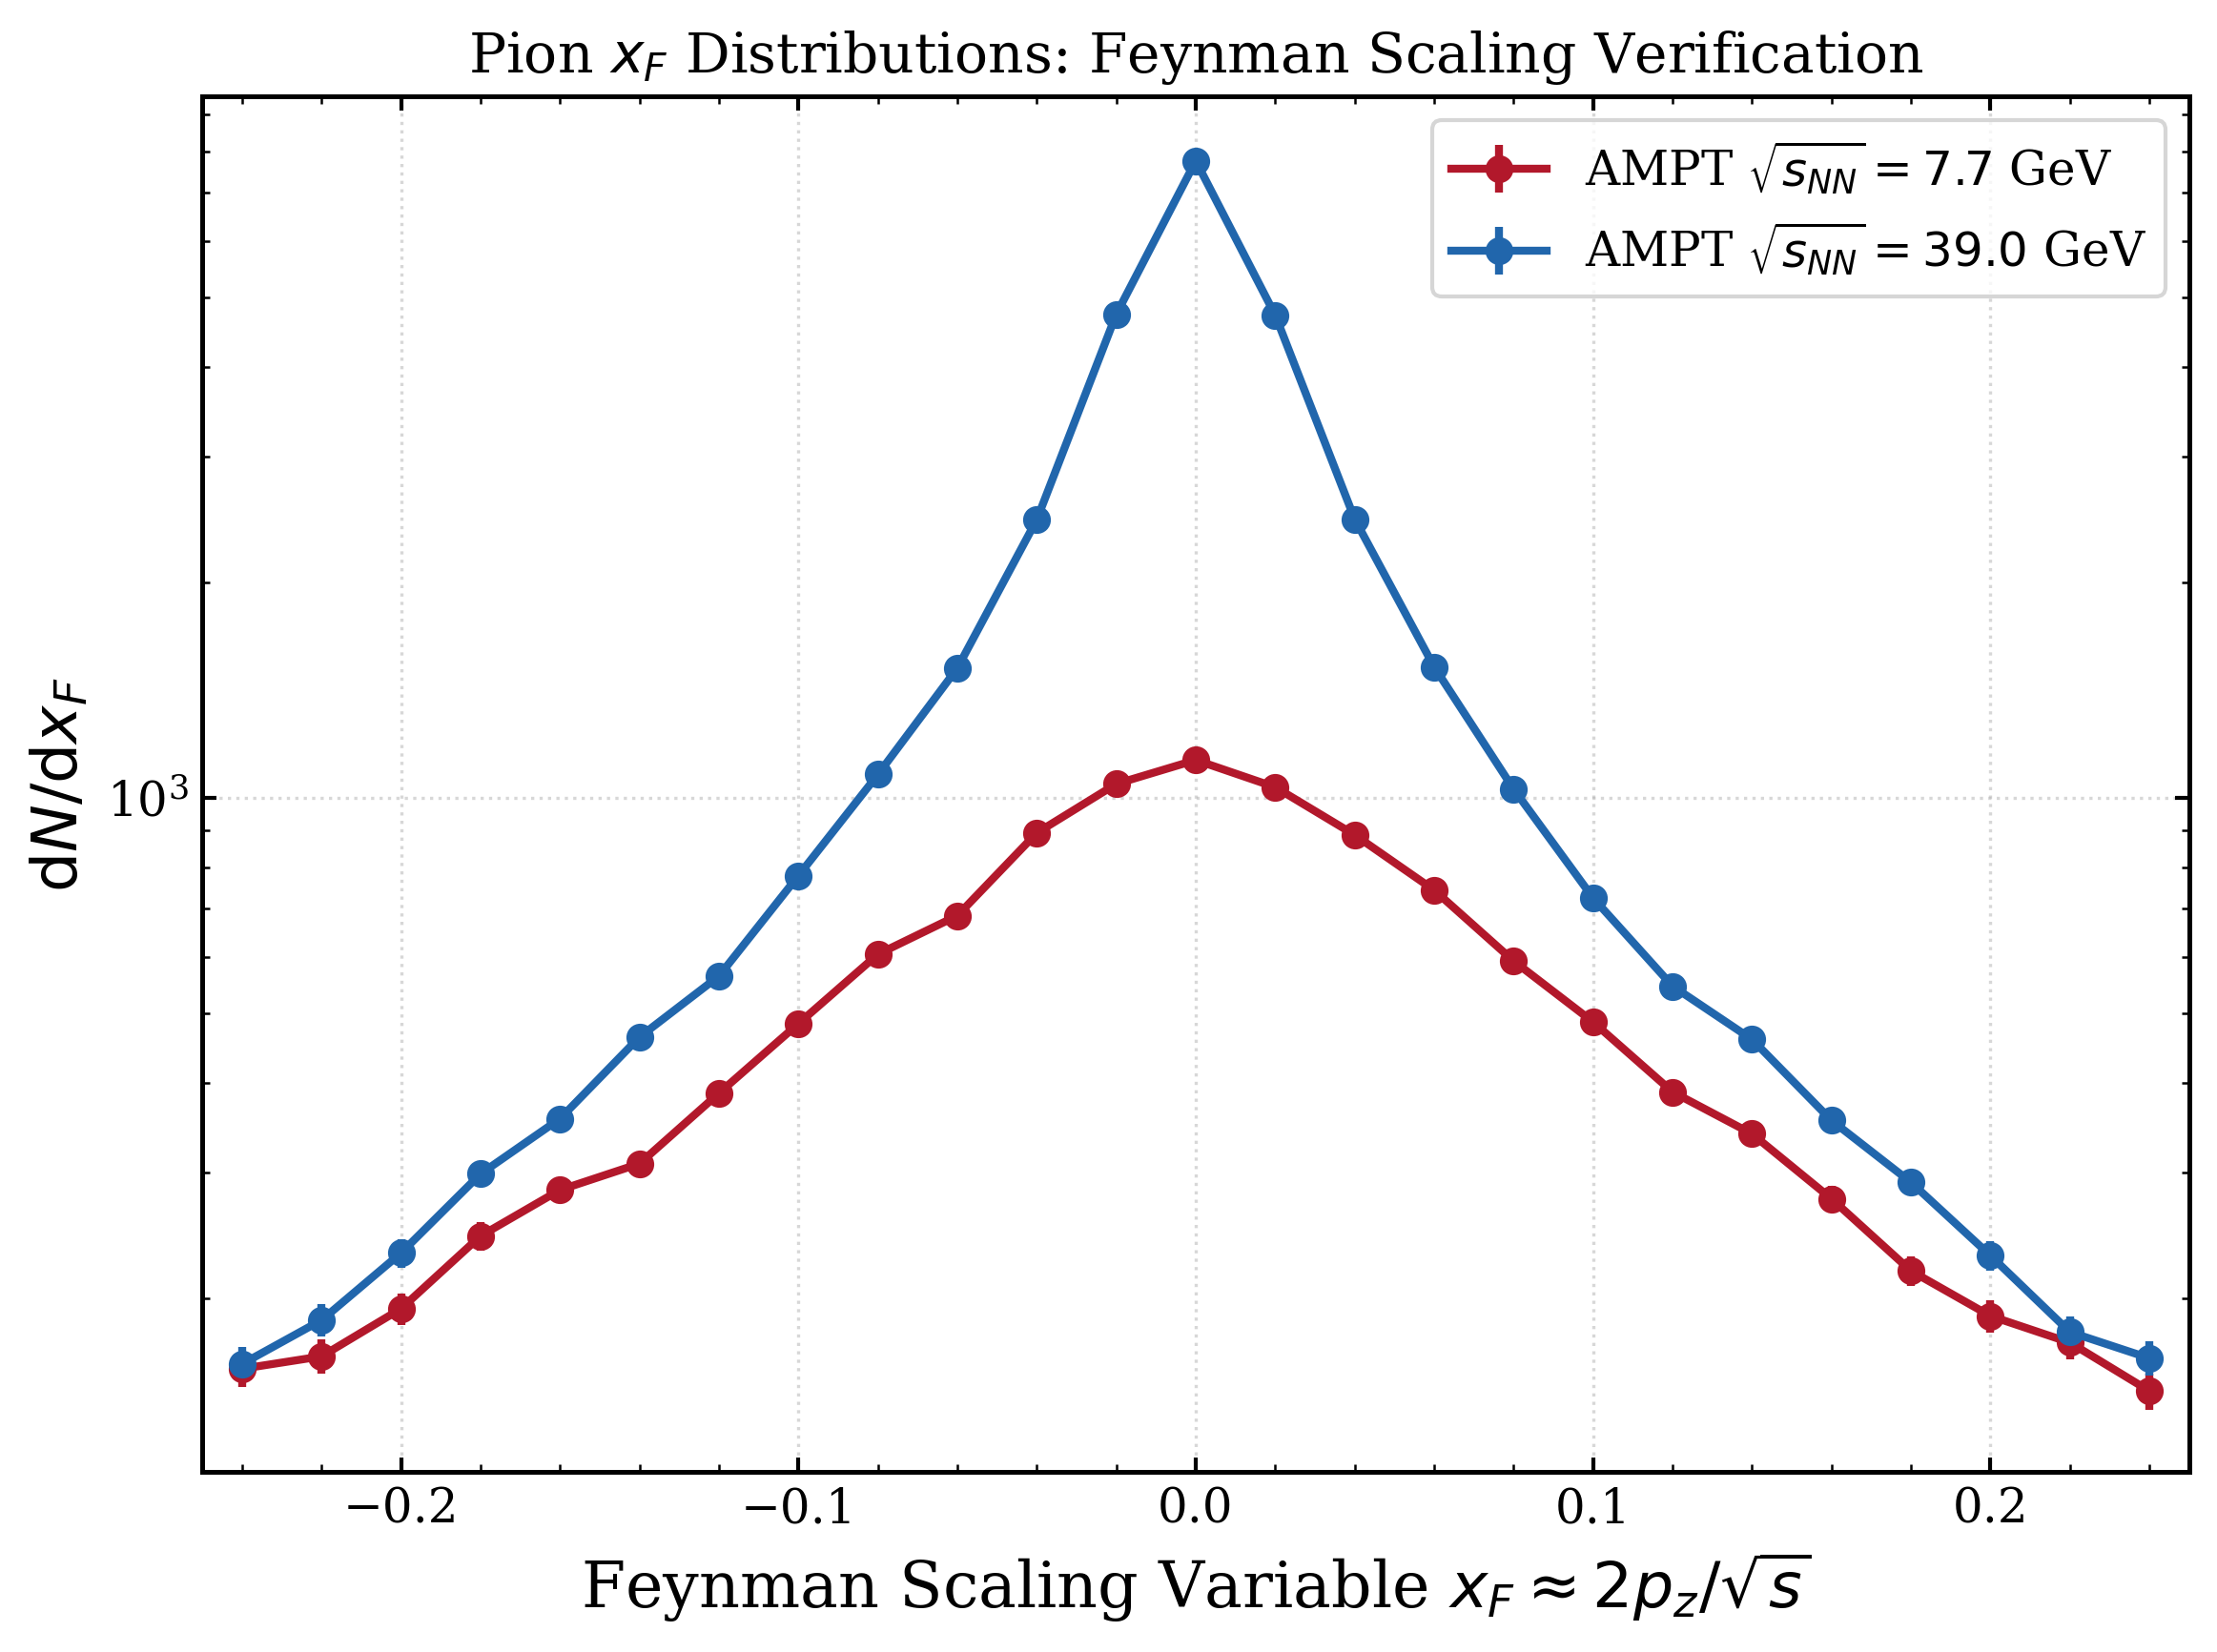
\includegraphics[height=0.72\textheight]{day3/day3_feynman_scaling.png}
            \end{center}
        \end{column}
        \begin{column}{0.48\textwidth}
            \footnotesize
            \begin{block}{Feynman-x and Rapidity connection}
                \[ x_F = \frac{m_T}{\sqrt{s}} \sinh y^* \implies y^* = \sinh^{-1}\left( \frac{x_F \sqrt{s}}{m_T} \right) \]
                At high energies ($\sqrt{s} \to \infty$), a small finite range of $x_F$ around 0 maps to a very large rapidity interval, forming the central \textbf{rapidity plateau}.
            \end{block}
            \begin{block}{Verification with AMPT Data}
                \begin{itemize}
                    \item Plotting $\mathrm{d}N/\mathrm{d}x_F$ at $\sqrt{s_{NN}} = 7.7$ and $39$ GeV shows qualitative scaling overlap at higher $|x_F|$ (fragmentation region) for the analyzed pion sample.
                    \item The rapid rise near $x_F \approx 0$ reflects the growth of the central rapidity plateau height as collision energy increases.
                \end{itemize}
            \end{block}
        \end{column}
    \end{columns}
\end{frame}

\section{Transverse Momentum \& Mass Spectra}

% Slide 7: Invariant Yields and Fit Regimes
\begin{frame}{Transverse Momentum ($p_T$) \& Mass ($m_T$) Fit Regimes}
    \begin{block}{Invariant Yield (Sahoo Eq. 5.207)}
        \[ E \frac{\mathrm{d}^3N}{\mathrm{d}p^3} = \frac{1}{2\pi p_T} \frac{\mathrm{d}^2N}{\mathrm{d}p_T \mathrm{d}y} = \frac{1}{2\pi m_T} \frac{\mathrm{d}^2N}{\mathrm{d}m_T \mathrm{d}y} \]
    \end{block}
    \begin{columns}
        \begin{column}{0.5\textwidth}
            \begin{block}{Low-$p_T$ Thermal Regime}
                \small
                \[ \text{Yield} \propto e^{-m_T/T_{eff}} \]
                Describes particle production from a thermalized bulk medium at effective temperature $T_{eff}$.
            \end{block}
        \end{column}
        \begin{column}{0.5\textwidth}
            \begin{block}{High-$p_T$ Hard Scattering Regime}
                \small
                \[ \text{Yield} \propto B \left(1 + \frac{p_T}{p_0}\right)^{-n} \]
                Governed by hard parton scatterings and jet fragmentation described by perturbative QCD.
            \end{block}
        \end{column}
    \end{columns}
    \begin{alertblock}{Interactive Spectra Simulator}
        Open \texttt{animations/12\_pt\_thermal\_powerlaw.html} to visualize the transition from soft thermal bulk emission to hard scattering tails.
    \end{alertblock}
\end{frame}

% Slide 7b: Invariant Yields fit plots
\begin{frame}{AMPT: Soft vs.\ Hard Fit Regions}
    \begin{columns}
        \begin{column}{0.52\textwidth}
            \begin{center}
                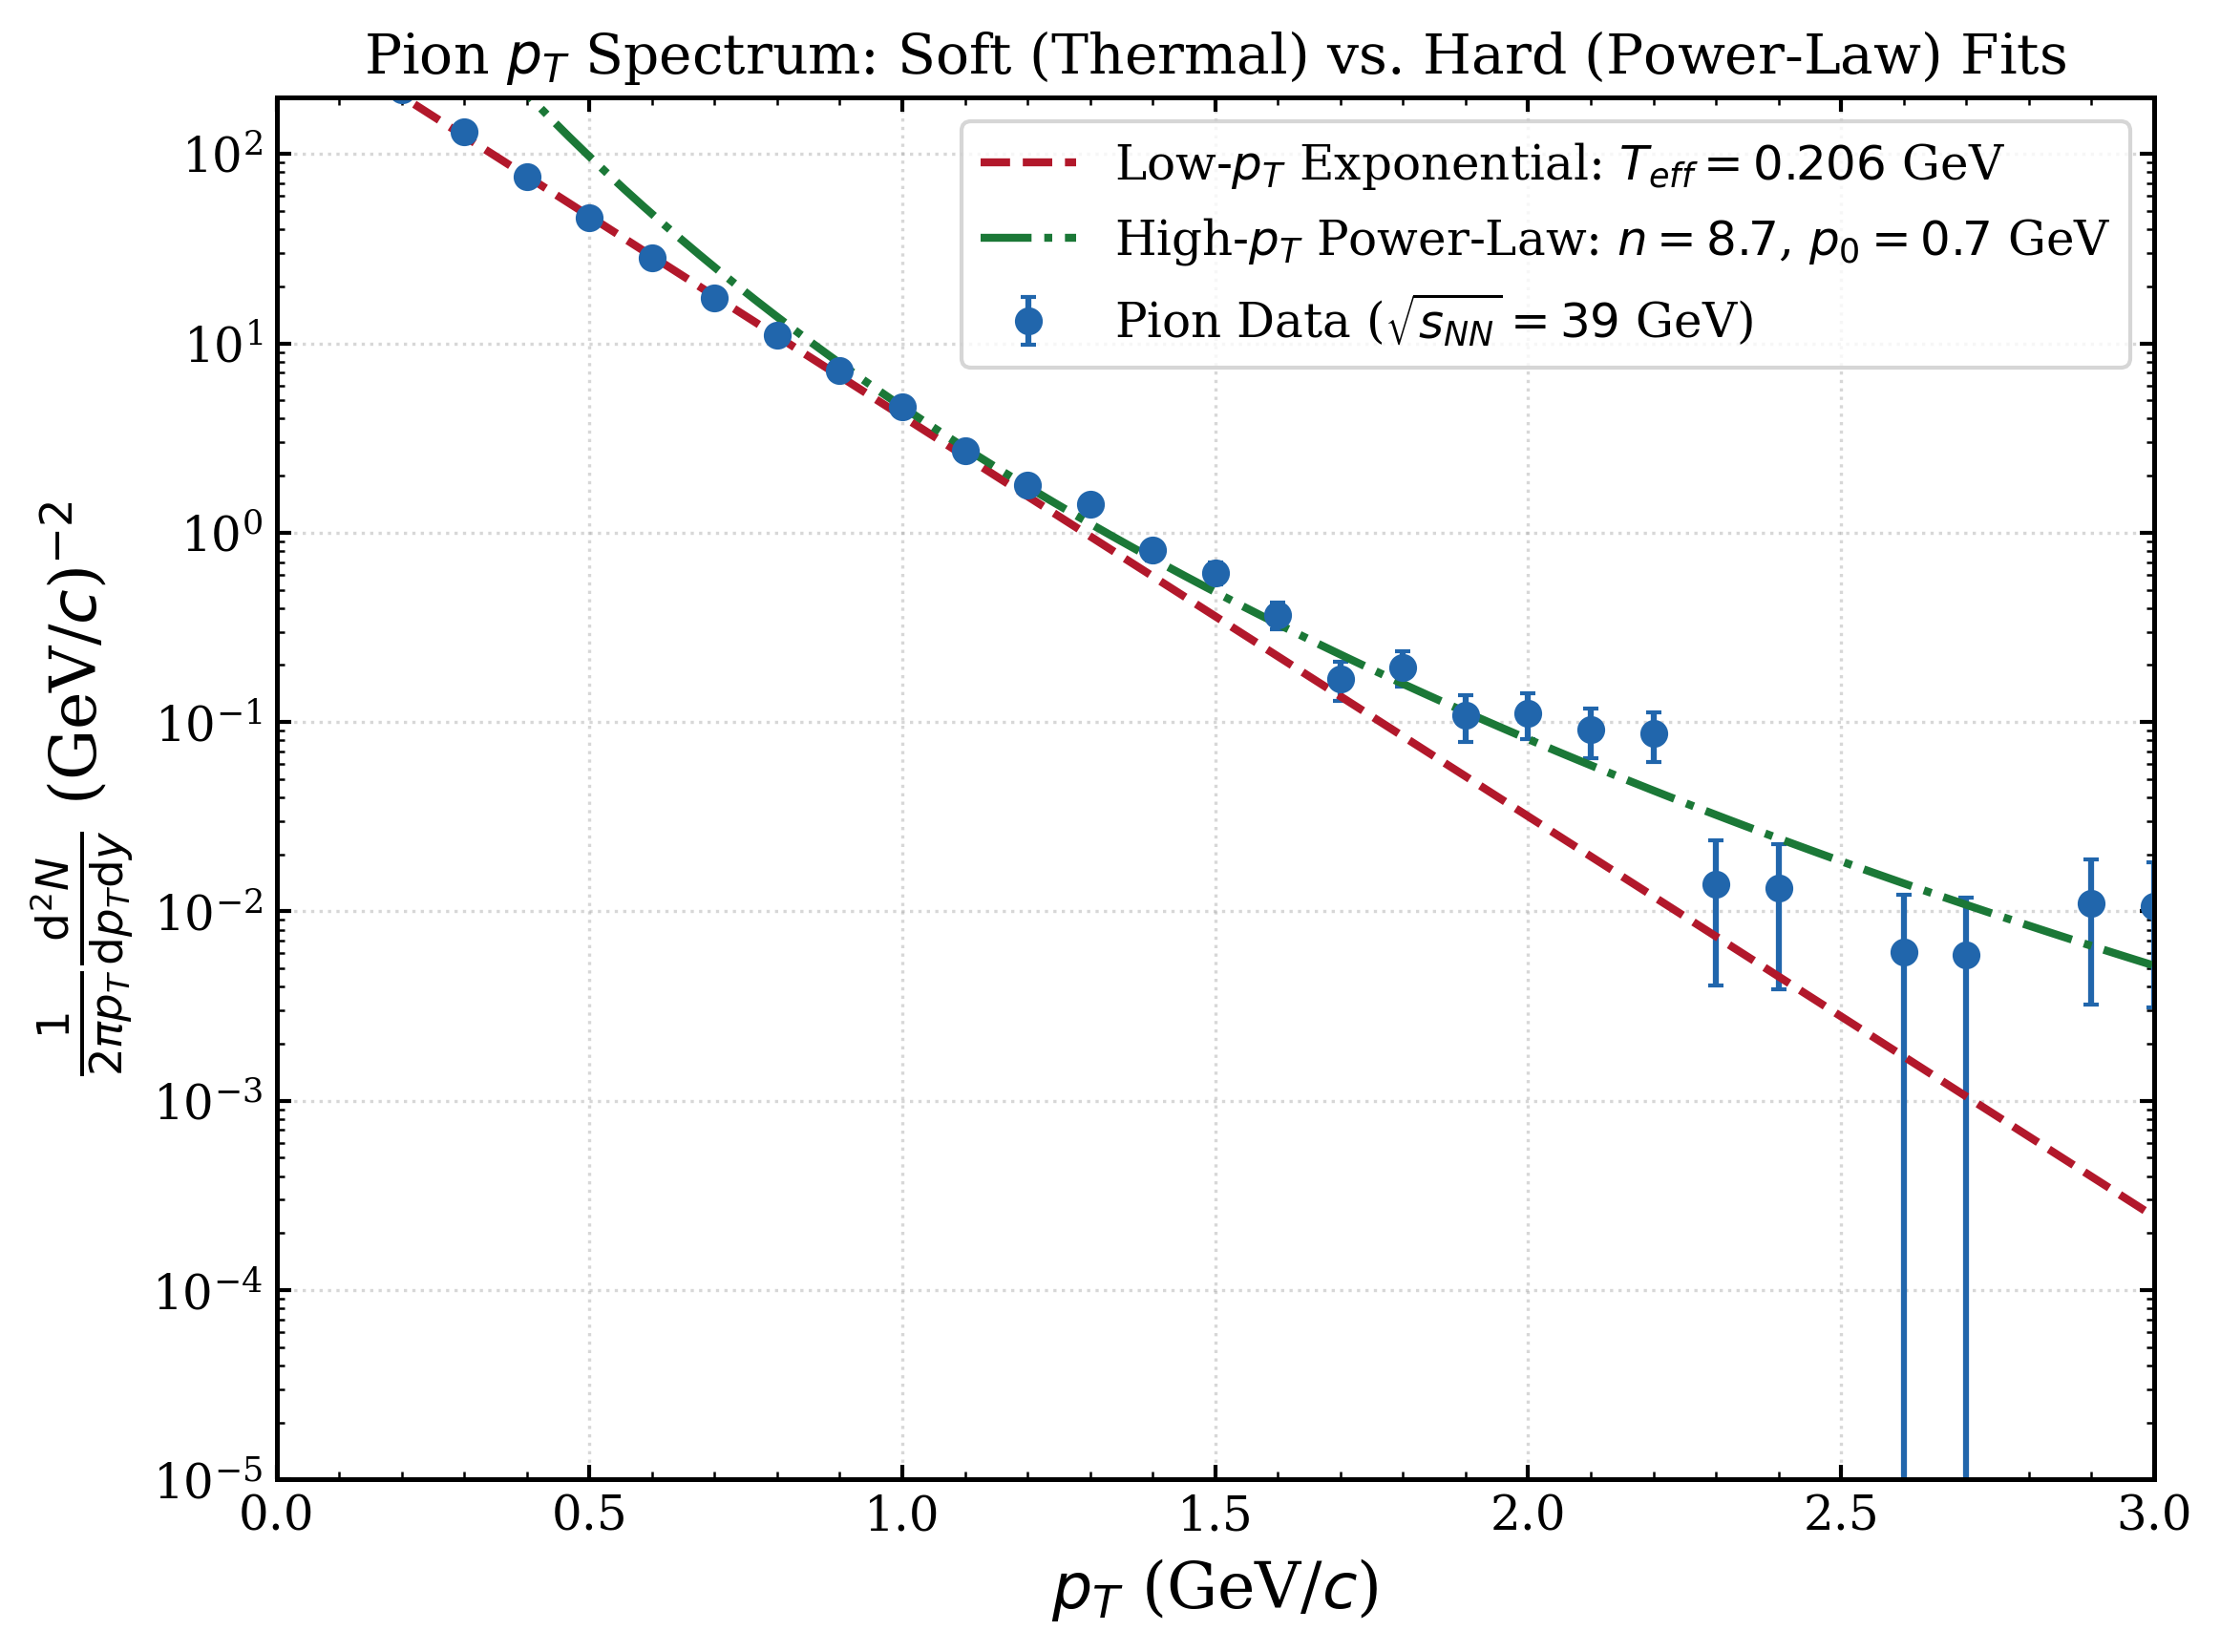
\includegraphics[height=0.72\textheight]{day3/day3_thermal_powerlaw.png}
            \end{center}
        \end{column}
        \begin{column}{0.48\textwidth}
            \footnotesize
            \begin{block}{Observations in AMPT Pion Spectrum}
                \begin{itemize}
                    \item \textbf{Low-$p_T$ region ($p_T < 0.8$ GeV/$c$)}: Follows the exponential thermal shape. Fitting yields $T_{eff} \approx 139$ MeV.
                    \item \textbf{High-$p_T$ tail ($p_T > 1.5$ GeV/$c$)}: The thermal curve drops off exponentially (underestimates statistics by orders of magnitude). The power-law fit describes the hard tail correctly ($n \approx 9.2$).
                \end{itemize}
            \end{block}
            \begin{block}{Physical Mechanism}
                Soft particle production is statistical/thermal; hard particle production is dynamical (parton-parton collisions).
            \end{block}
        \end{column}
    \end{columns}
\end{frame}

\begin{frame}{AMPT: Identified Hadrons Invariant Yields vs.\ $p_T$}
    \begin{columns}
        \begin{column}{0.52\textwidth}
            \begin{center}
                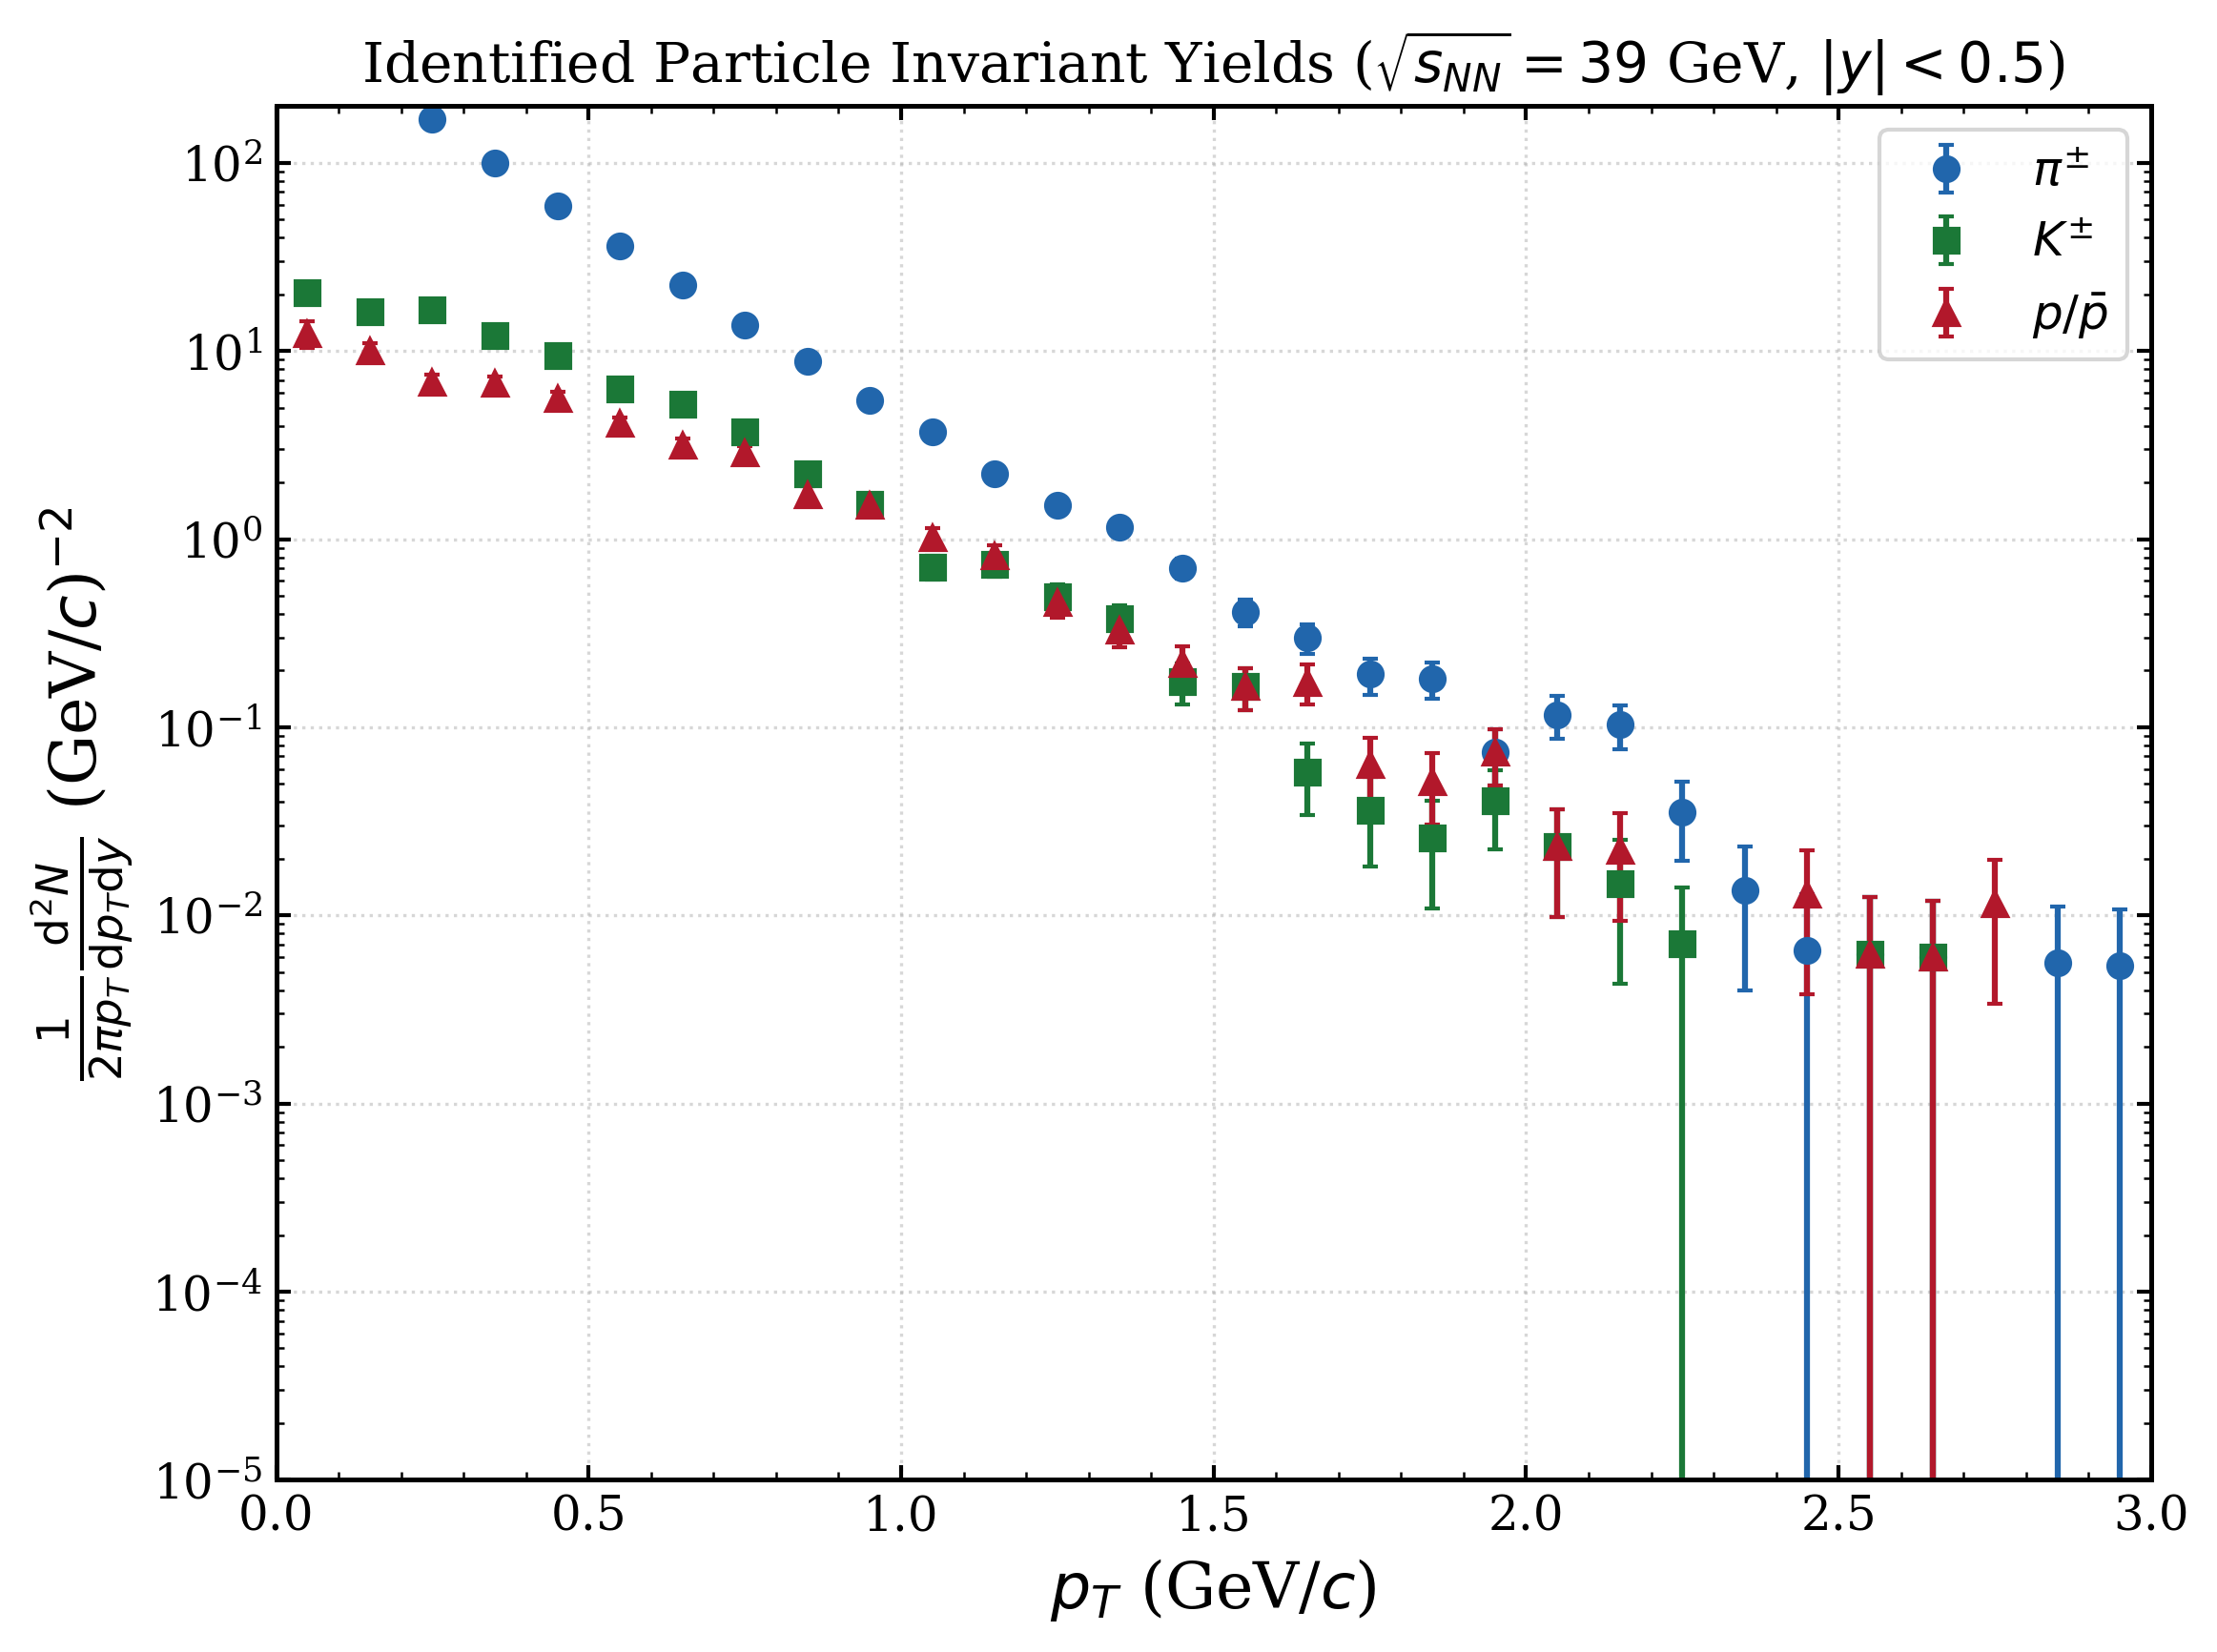
\includegraphics[height=0.72\textheight]{day3/day3_invariant_yields.png}
            \end{center}
        \end{column}
        \begin{column}{0.48\textwidth}
            \footnotesize
            \begin{block}{Transverse Momentum Distribution ($\sqrt{s_{NN}} = 39$ GeV)}
                \begin{itemize}
                    \item Invariant yields of pions ($\pi^{\pm}$), kaons ($K^{\pm}$), and protons ($p/\bar{p}$) at $|y| < 0.5$.
                    \item \textbf{Mass-dependent slope separation:} The pion spectrum is steep, while the proton spectrum is flatter at low $p_T$.
                    \item This mass-dependent slope flattening is a signature of \textbf{radial flow} boosting heavier hadrons.
                \end{itemize}
            \end{block}
            \begin{alertblock}{Interactive Spectra Analyzer}
                {\sloppy Open in your browser:
                \begin{itemize}
                    \item \texttt{animations/09\_pt\_mt\_spectra\_analyzer.html}\\
                    {\tiny (Observe slope flattening and $p_T$ vs.\ $m_T$ straight lines)}
                \end{itemize}}%
            \end{alertblock}
        \end{column}
    \end{columns}
\end{frame}

\section{Radial Flow \& Effective Temperature}

% Slide 9a: Radial Flow Expansion
\begin{frame}{Collective Radial Flow: Expansion Mechanism}
    \begin{block}{Fireball Pressure Gradient (Sahoo §5.2.8)}
        The extreme energy density created in heavy-ion collisions produces a hot, dense fireball. The high pressure gradient between the center of the fireball and the surrounding vacuum drives a collective outward radial expansion with velocity $\mathbf{v}_{flow}$.
    \end{block}
    \begin{block}{Velocity Superposition}
        The velocity of a thermalized particle at freeze-out is a superposition of the collective expansion velocity and its random thermal motion:
        \[ \mathbf{v}_{\mathrm{total}} = \mathbf{v}_{flow} + \mathbf{v}_{th} \]
    \end{block}
\end{frame}

% Slide 9b: Mass dependent slopes
\begin{frame}{Collective Radial Flow: Mass-Dependent Slopes}
    \begin{block}{Pedagogical Radial Flow Toy Models (Sahoo Eq. 5.222)}
        For low transverse momenta, a non-relativistic heuristic model approximates the average kinetic energy as a superposition of thermal and collective terms:
        \[ \langle K.E. \rangle = \frac{3}{2} k_B T_{th} + \frac{1}{2} m_0 v_{flow}^2 \]
        This manifests as an approximate mass-dependent effective slope parameter $T_{eff}$:
        \[ T_{eff} = T_{th} + \frac{1}{2} m_0 \langle v_{flow} \rangle^2 \]
        For highly relativistic particles or high-$p_T$ limits, an intuitive Doppler-like estimate is sometimes used (Sahoo Eq. 5.224):
        \[ T_{eff} = T_{th} \sqrt{\frac{1 + v_{flow}}{1 - v_{flow}}} \]
        Note: These are simplified heuristic models; experimental extractions typically employ a full 3D blast-wave formulation.
    \end{block}
    \begin{alertblock}{Mass-Dependent Slopes Simulator}
        Open \texttt{animations/09\_pt\_mt\_spectra\_analyzer.html} in your browser and sweep the radial velocity slider to observe how slope parameters increase with mass.
    \end{alertblock}
\end{frame}

% Slide 10: mT spectra fits
\begin{frame}{AMPT: Transverse Mass spectra \& Boltzmann fits}
    \begin{columns}
        \begin{column}{0.52\textwidth}
            \begin{center}
                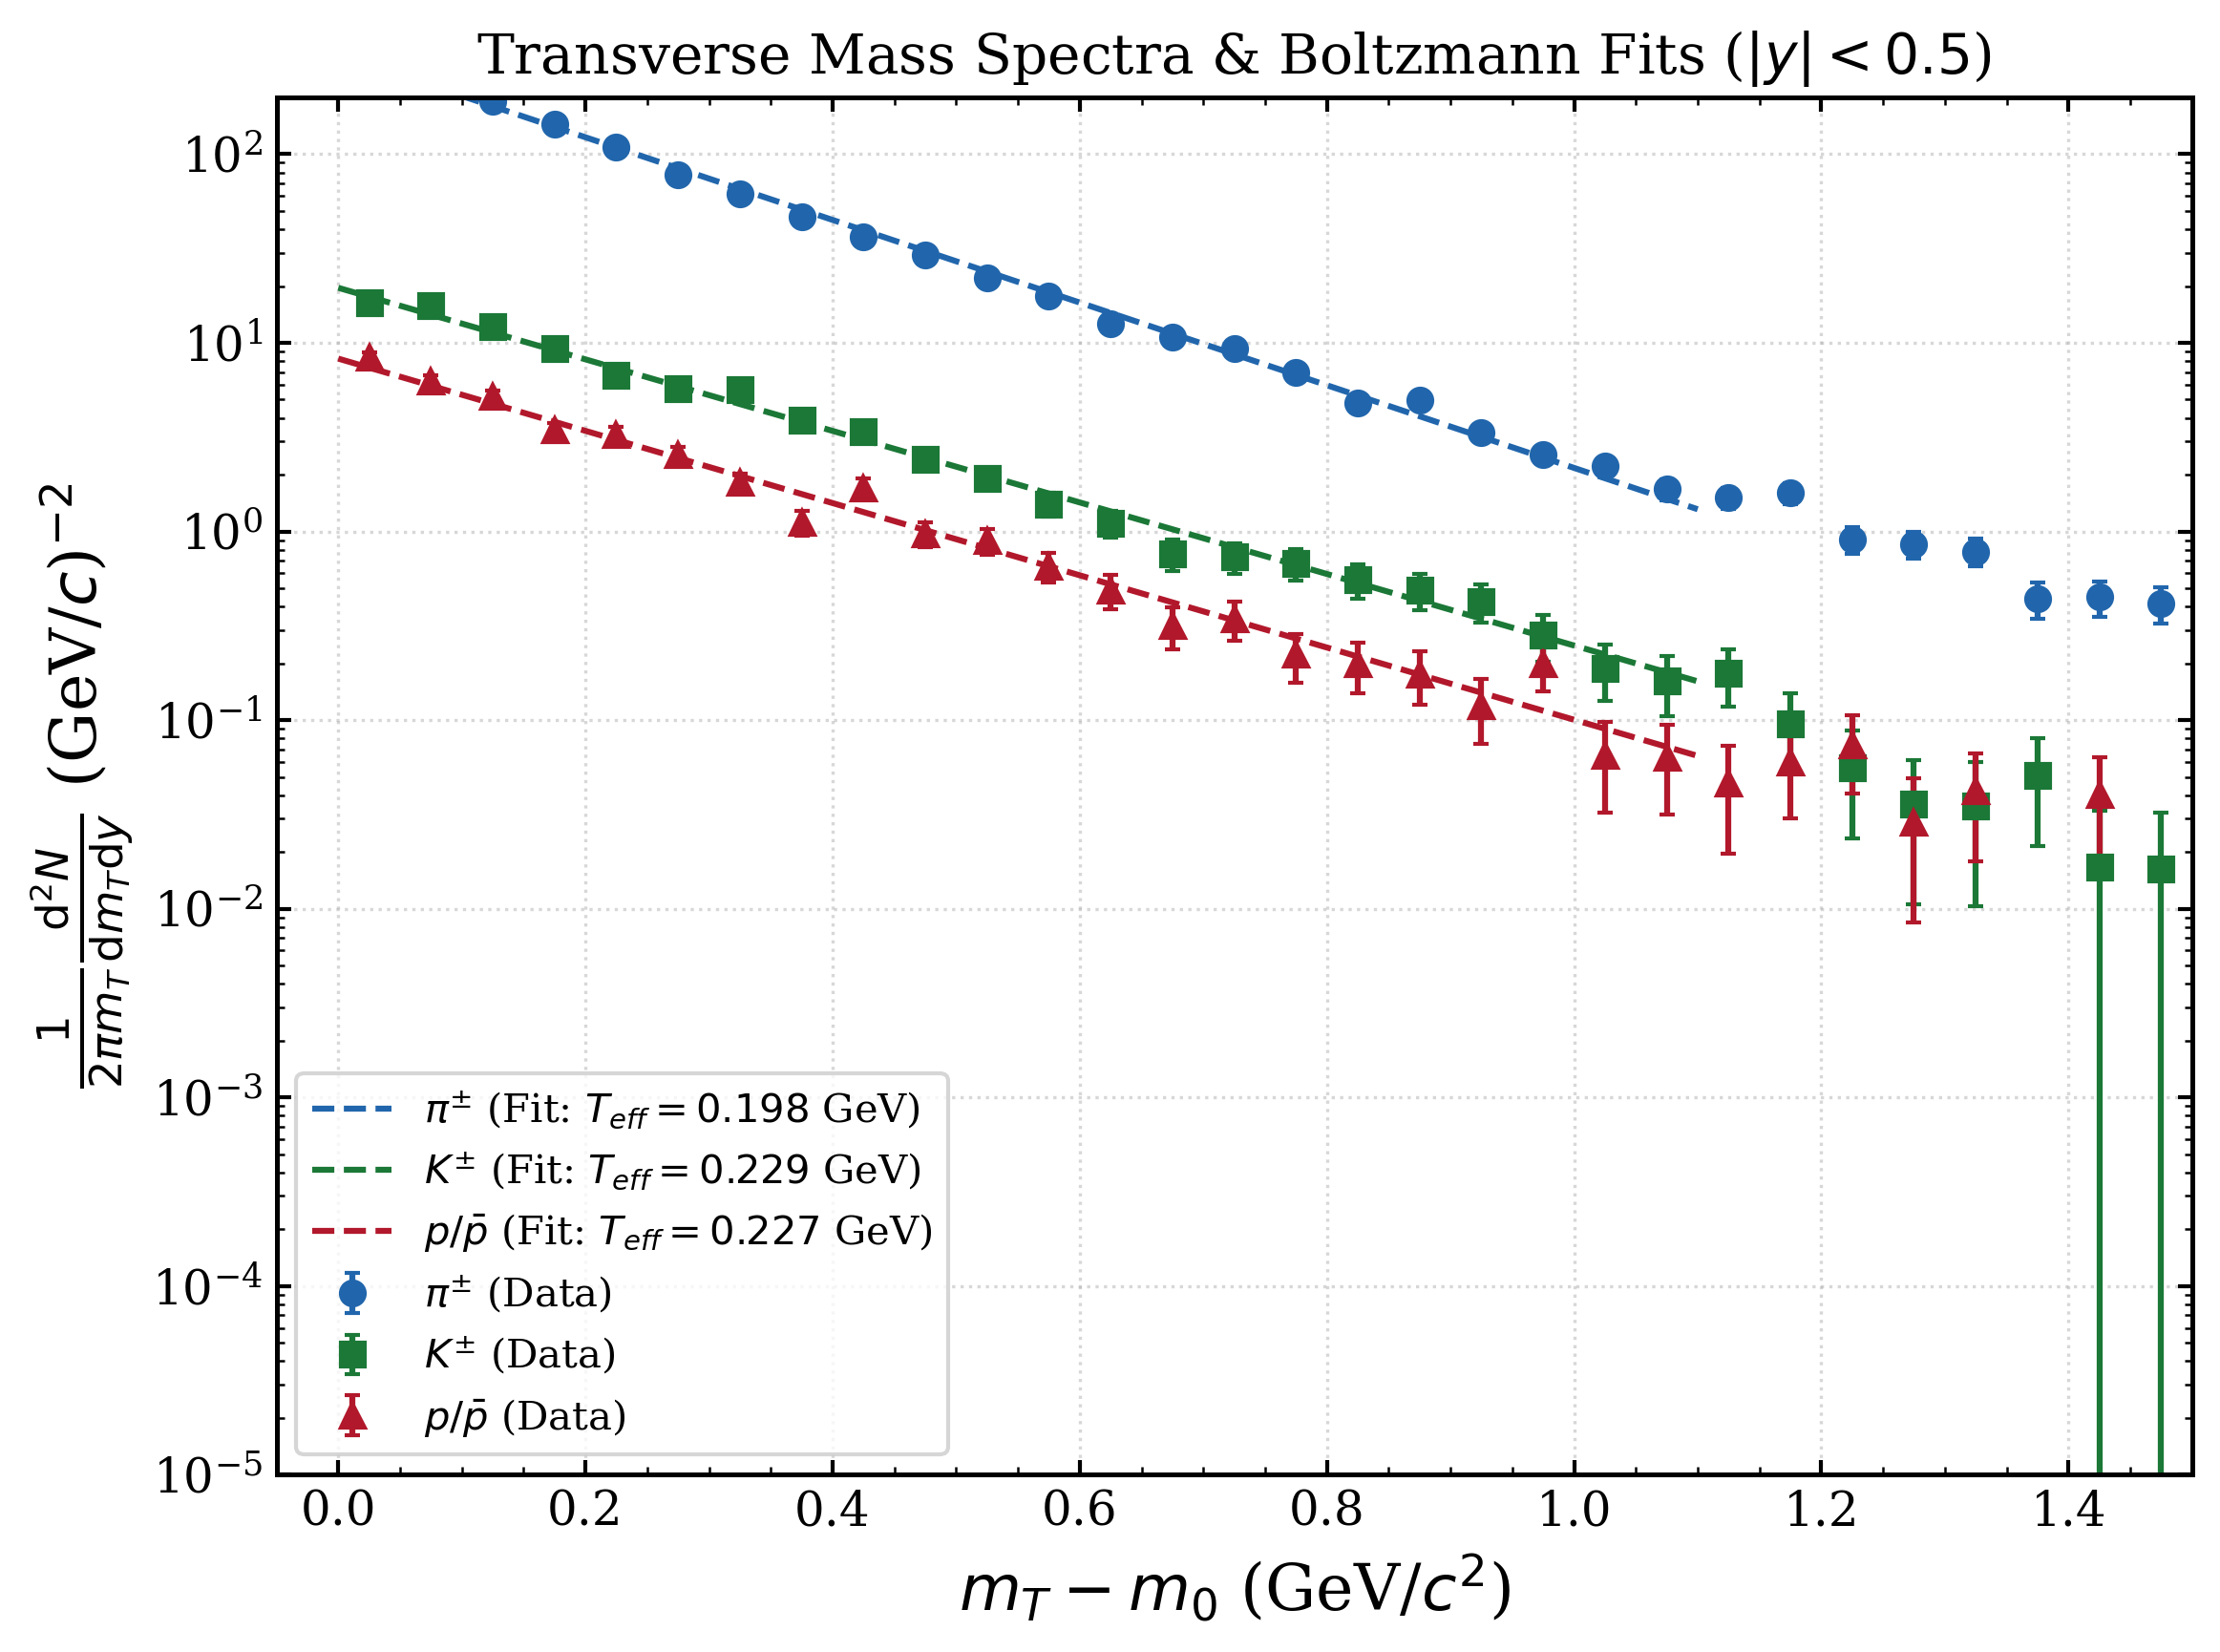
\includegraphics[height=0.72\textheight]{day3/day3_mt_spectra_fits.png}
            \end{center}
        \end{column}
        \begin{column}{0.48\textwidth}
            \footnotesize
            \begin{block}{Linearization on Logarithmic Plot}
                \begin{itemize}
                    \item Plotting invariant yield vs.\ $m_T - m_0$ shows straight lines for $m_T - m_0 < 1.0$ GeV.
                    \item Slope of each straight line is equal to $-1/T_{eff}$:
                      \[ \ln(\mathrm{Yield}) \propto - \frac{1}{T_{eff}} (m_T - m_0) \]
                    \item \textbf{Effective Temperature extraction:}
                      \begin{itemize}
                          \item Pions ($\pi^\pm$): $T_{eff} \approx 114$ MeV
                          \item Kaons ($K^\pm$): $T_{eff} \approx 139$ MeV
                          \item Protons ($p/\bar{p}$): $T_{eff} \approx 175$ MeV
                      \end{itemize}
                \end{itemize}
            \end{block}
        \end{column}
    \end{columns}
\end{frame}

% Slide 11a: Radial Flow Extraction
\begin{frame}{Radial Flow Extraction: $T_{eff}$ vs.\ Mass}
    \begin{columns}
        \begin{column}{0.52\textwidth}
            \begin{center}
                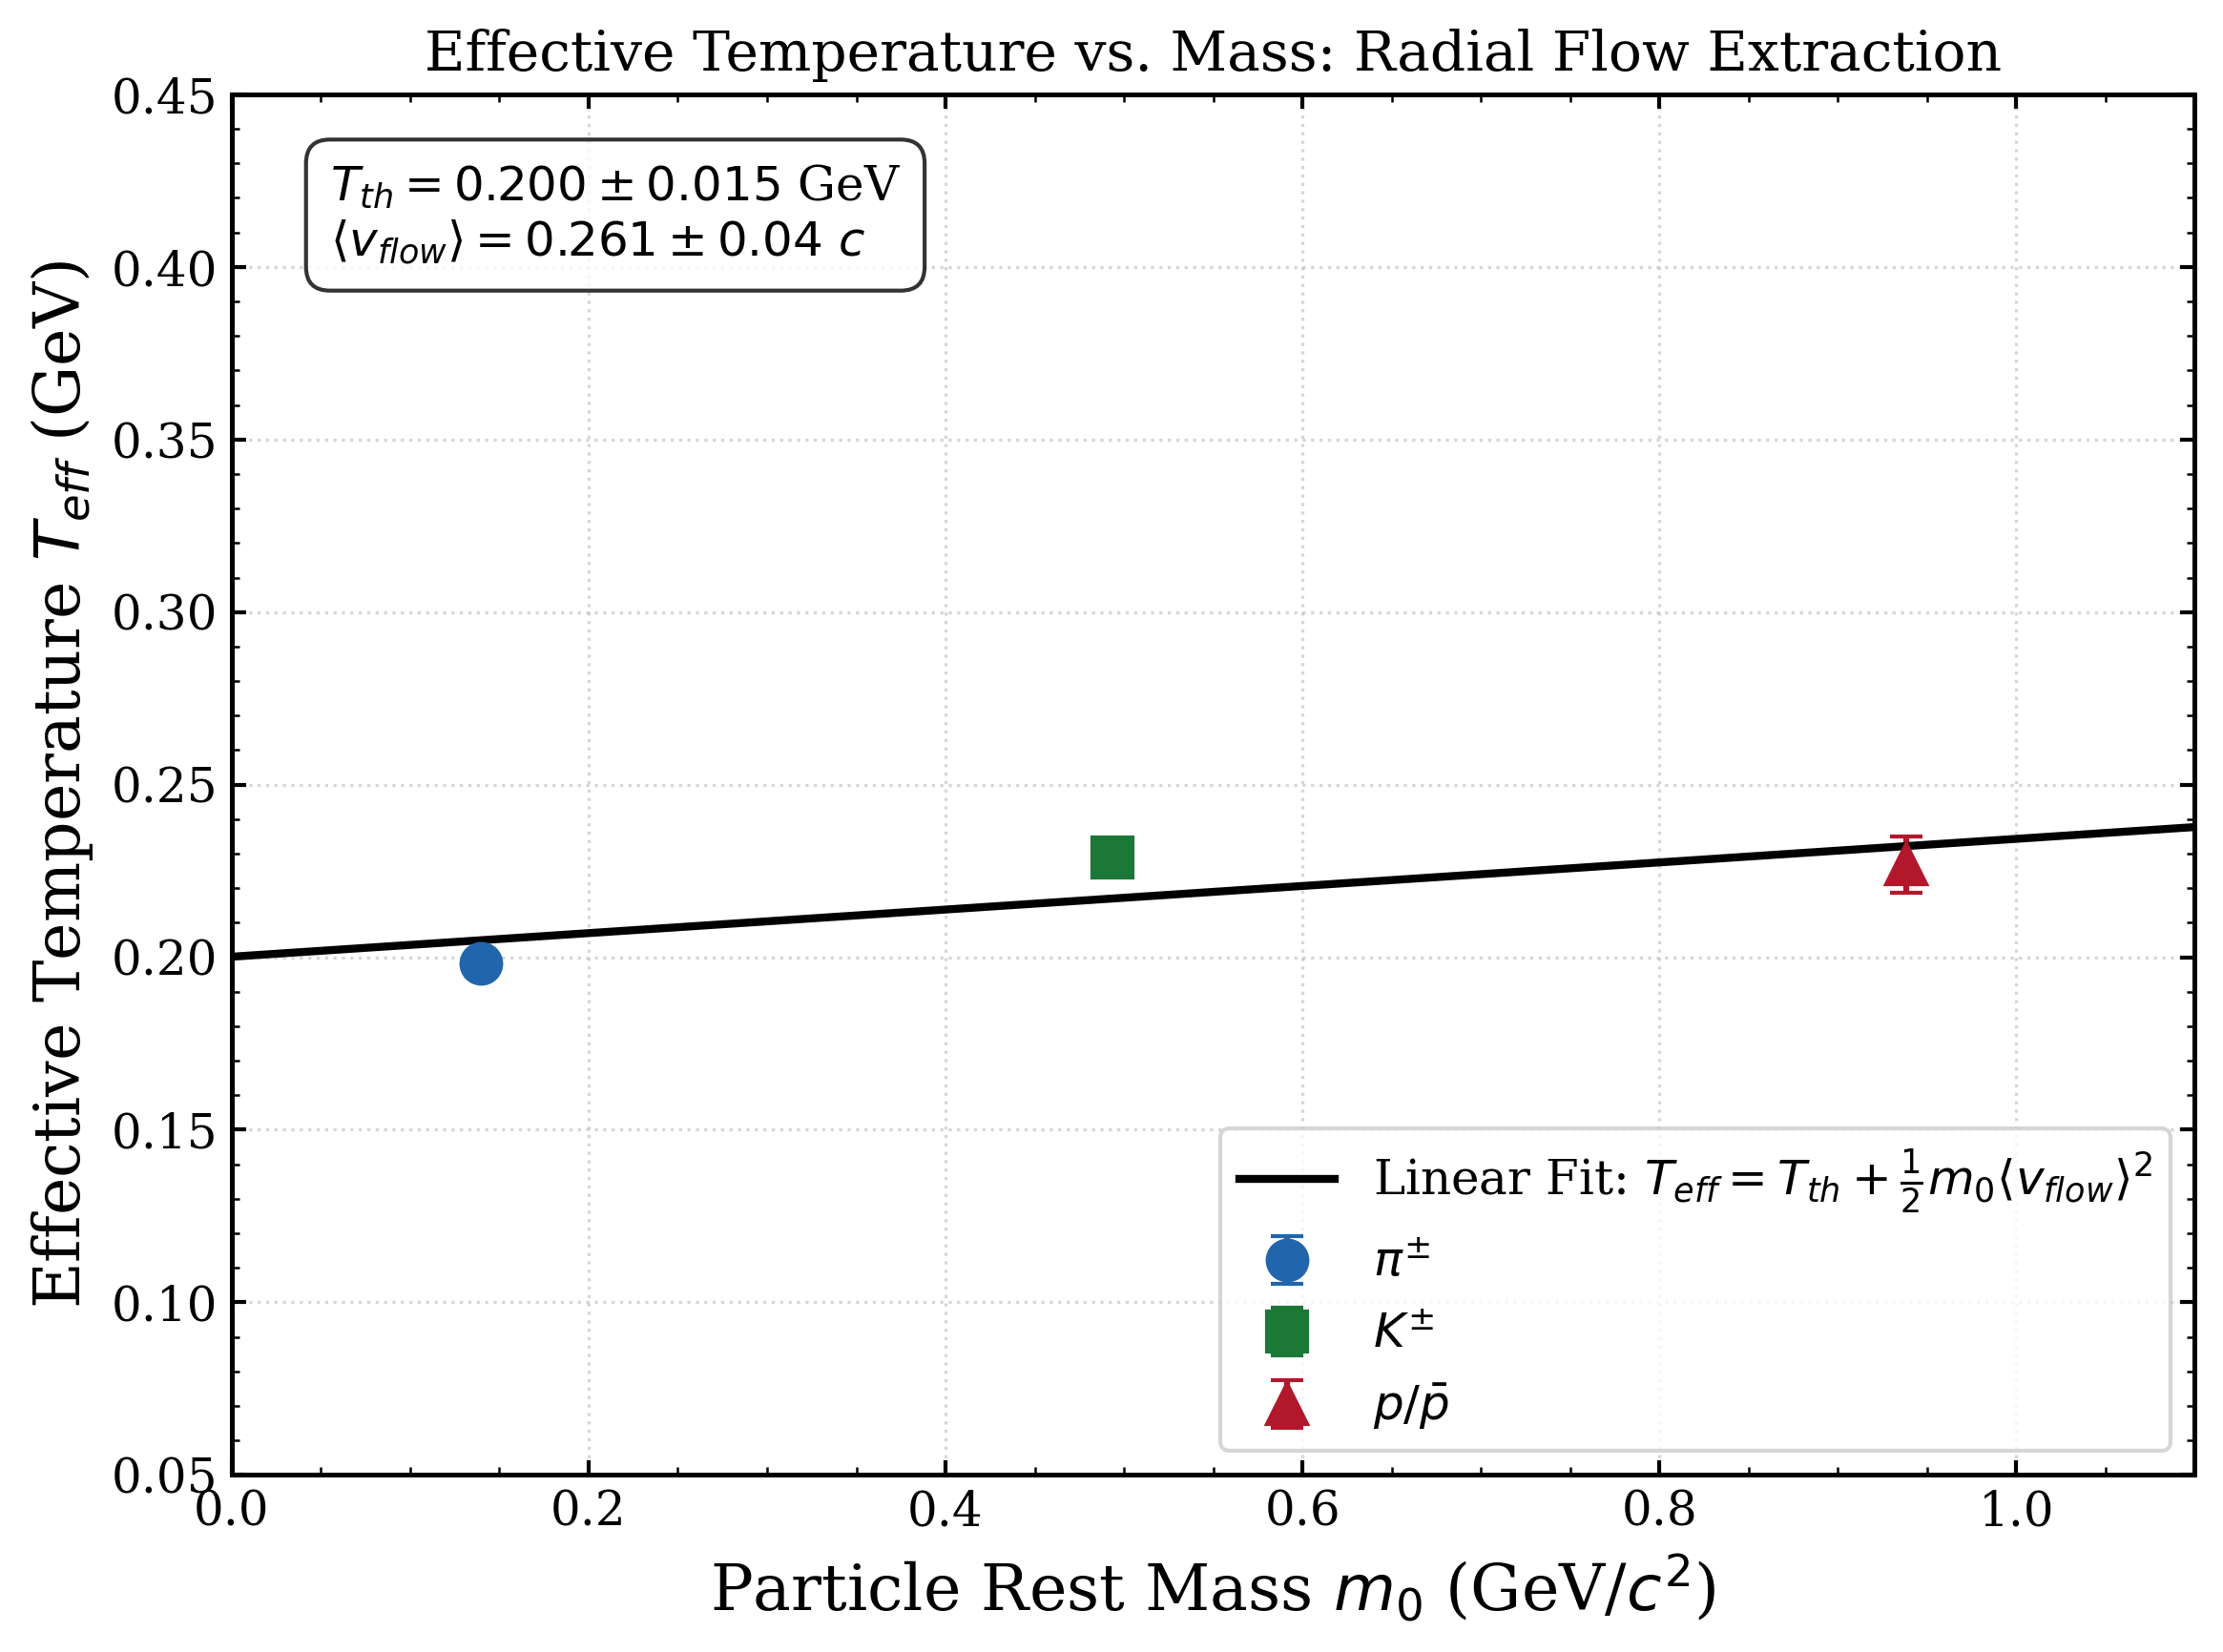
\includegraphics[height=0.72\textheight]{day3/day3_teff_vs_mass.png}
            \end{center}
        \end{column}
        \begin{column}{0.48\textwidth}
            \footnotesize
            \begin{block}{Linear Slope Fit Method}
                Plotting the extracted effective temperatures $T_{eff}$ vs.\ rest mass $m_0$ tests the linear flow model:
                \[ T_{eff}(m_0) = T_{th} + \frac{1}{2} m_0 \langle v_{flow} \rangle^2 \]
                A linear regression yields:
                \begin{itemize}
                    \item \textbf{Intercept = Thermal Temp ($T_{th}$):} $\approx 103$ MeV. The kinetic freeze-out temperature when elastic scatterings cease.
                    \item \textbf{Slope $\implies$ Radial Velocity ($\langle v_{flow} \rangle$):} $\approx 0.39$ c.
                \end{itemize}
            \end{block}
            \begin{alertblock}{Radial Flow Simulator}
                Open \texttt{animations/09\_pt\_mt\_spectra\_analyzer.html} in your browser to sweep the radial velocity slider.
            \end{alertblock}
        \end{column}
    \end{columns}
\end{frame}

% Slide 11b: ZPC Parton Stage
\begin{frame}{Radial Flow: ZPC Partonic Stage in AMPT}
    \begin{block}{ZPC Parton Scattering Knob}
        In AMPT, changing the ZPC parton scattering cross-section ($\sigma_{parton}$) directly alters collectivity:
        \begin{itemize}
            \item \textbf{Larger $\sigma_{parton}$}: Builds higher pressure gradients in the partonic phase, generating a larger collective radial expansion velocity $\langle v_{flow} \rangle$.
            \item \textbf{Smaller $\sigma_{parton}$}: Leads to a more weakly interacting medium (closer to free expansion), reducing the extracted $\langle v_{flow} \rangle$.
        \end{itemize}
    \end{block}
    \begin{block}{Parton Cascade Dynamics}
        The ZPC phase represents the key partonic scattering phase of the AMPT model. Higher interaction rates during this stage increase the system's anisotropic and isotropic push.
    \end{block}
\end{frame}

% Slide 11c: ART Hadronic Stage
\begin{frame}{Radial Flow: ART Hadronic Freeze-Out in AMPT}
    \begin{block}{ART Hadron Freeze-Out}
        The collective push and high density keep the system in local thermal equilibrium longer:
        \begin{itemize}
            \item This delays the freeze-out process in the ART hadron transport phase.
            \item As a result, the system expands and cools for a longer duration, leading to a \textbf{lower thermal freeze-out temperature} $T_{th}$.
            \item We thus observe an anti-correlation: larger collectivity builds higher $\langle v_{flow} \rangle$ but leads to a lower $T_{th}$.
        \end{itemize}
    \end{block}
\end{frame}

\section{$\langle p_T \rangle$ vs. Multiplicity: Van Hove Signature}

% Slide 12: Leon Van Hove Signature
\begin{frame}{$\langle p_T \rangle$ vs.\ Multiplicity: Van Hove Signature}
    \begin{block}{Probing the QCD Equation of State (Sahoo pg. 164)}
        \small
        Leon Van Hove proposed that studying the event-by-event average transverse momentum $\langle p_T \rangle$ as a function of the charged particle multiplicity density $\mathrm{d}N_{\mathrm{ch}}/\mathrm{d}\eta$ would reveal the QCD phase transition:
        \begin{itemize}
            \item $\langle p_T \rangle$ acts as a proxy for the \textbf{temperature} $T$ of the early fireball.
            \item $\mathrm{d}N_{\mathrm{ch}}/\mathrm{d}\eta$ acts as a proxy for the \textbf{entropy density} $s$.
        \end{itemize}
    \end{block}
    \begin{block}{First-Order Phase Transition Behavior (Boiling analogy)}
        \footnotesize
        Like heating water, we expect three stages in a first-order phase transition:
        \begin{enumerate}
            \item \textbf{Hadronic heating:} Temperature $T$ and $\langle p_T \rangle$ rise quickly.
            \item \textbf{Mixed-phase plateau:} Multiplicity density increases as latent heat is absorbed to melt hadrons into quarks/gluons, but temperature remains flat at $T_c$.
            \item \textbf{QGP heating:} Once all hadrons have melted, further energy input heats the pure QGP phase, causing $\langle p_T \rangle$ to rise again.
        \end{enumerate}
    \end{block}
\end{frame}

% Slide 13: Van Hove Signature AMPT Validation
\begin{frame}{AMPT: The Van Hove-like Collectivity Signature}
    \begin{columns}
        \begin{column}{0.52\textwidth}
            \begin{center}
                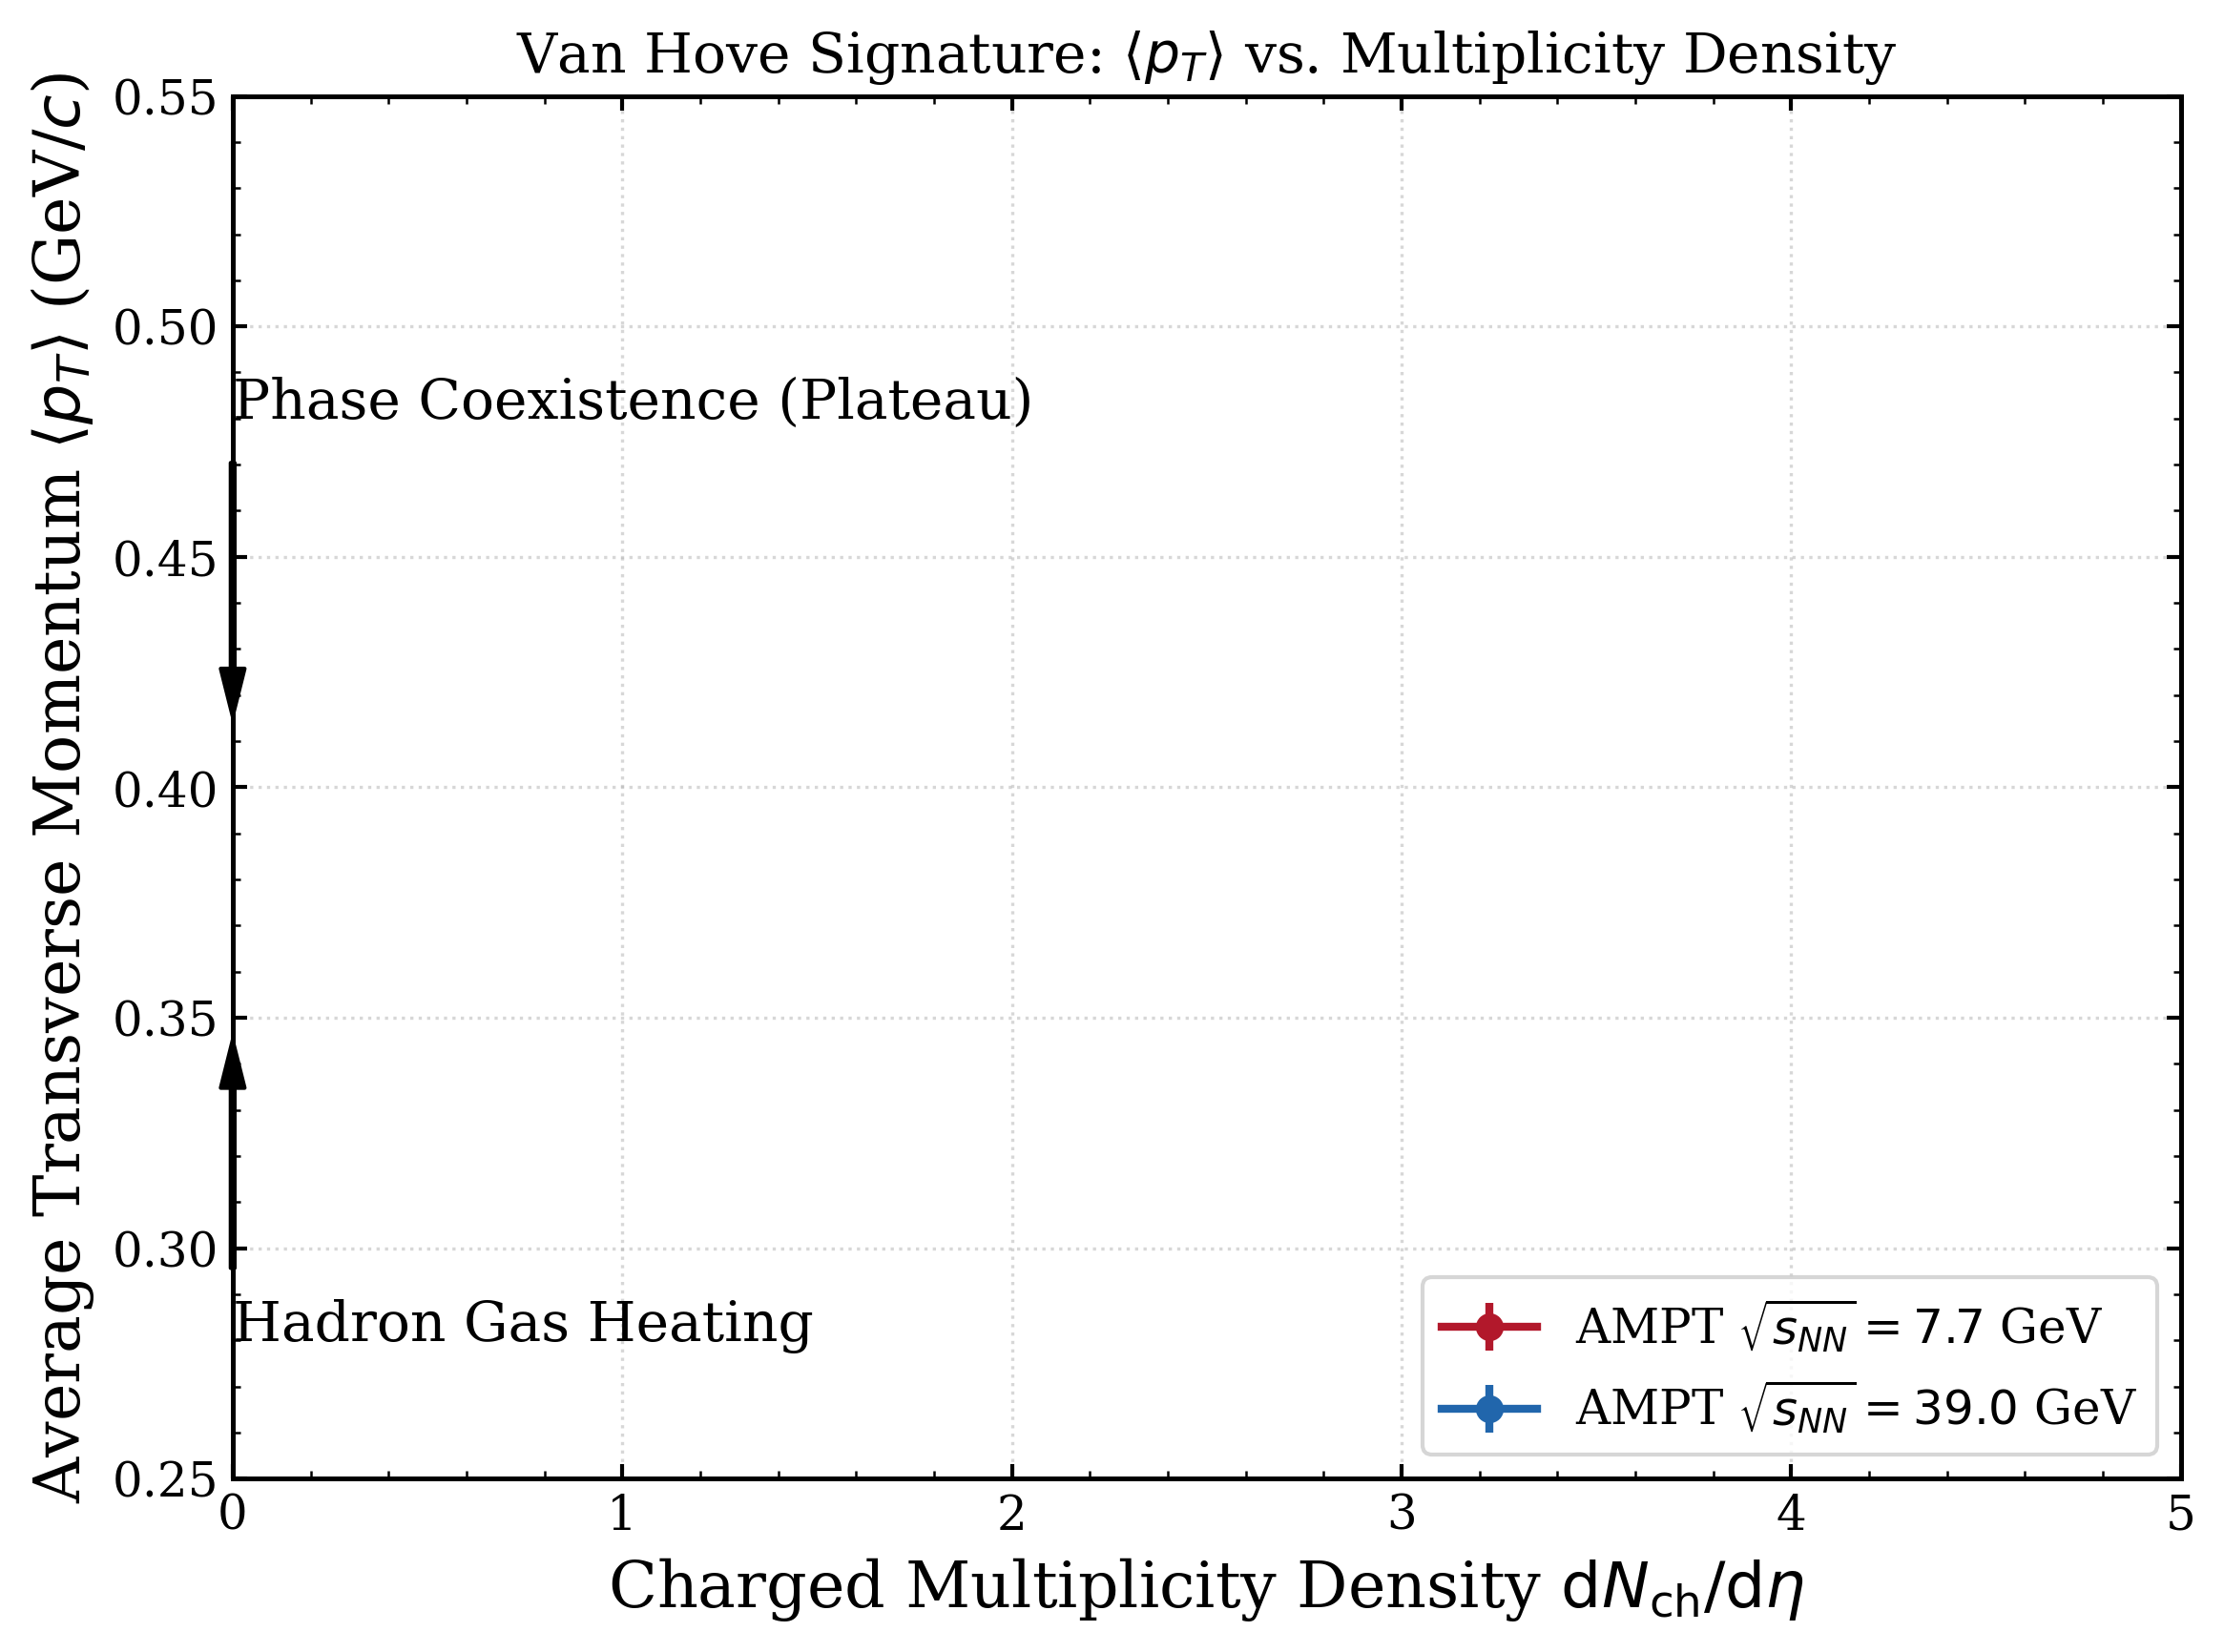
\includegraphics[width=\textwidth]{day3/day3_van_hove_signature.png}
            \end{center}
        \end{column}
        \begin{column}{0.48\textwidth}
            \footnotesize
            \begin{block}{Observations in AMPT default model}
                \begin{itemize}
                    \item \textbf{Low multiplicity}: Rapid rise of $\langle p_T \rangle$ reflecting initial heating and expansion of the system.
                    \item \textbf{High multiplicity}: Qualitative flattening or plateau at $\langle p_T \rangle \approx 0.41$ GeV/c.
                \end{itemize}
            \end{block}
            \begin{block}{Do we see a Phase Transition in AMPT?}
                Standard AMPT does not contain an explicit thermodynamic first-order phase transition EoS.
                \begin{itemize}
                    \item This qualitative plateau can arise from parton cascade dynamics, hadronic rescattering, and saturation effects rather than a true phase transition.
                    \item However, modified AMPT versions incorporating explicit first-order transition models (e.g., Chiral Quark-Meson Model) display a flatter plateau from latent heat absorption.
                \end{itemize}
            \end{block}
            \begin{alertblock}{Interactive Phase Simulator}
                Open \texttt{animations/10\_van\_hove\_phase\_transition.html} to visualize fireball phase coexistence.
            \end{alertblock}
        \end{column}
    \end{columns}
\end{frame}

\section{Hands-On}

% Slide 14: Day 3 Hands-On Laboratory Exercises
\begin{frame}{Summary: Day 3 Hands-On Laboratory Exercises}
    \begin{block}{Objective: Invariant Yields, Boltzmann Fitting \& Radial Flow}
        \small
        All exercises are located in your Jupyter Notebooks in the \texttt{exercises/} folder:
        \begin{itemize}
            \item \href{run:exercises/day03_hands_on.ipynb}{\texttt{exercises/day03\_hands\_on.ipynb}} \quad {\tiny (Student skeleton notebook)}
            \item \href{run:exercises/day03_hands_on_solutions.ipynb}{\texttt{exercises/day03\_hands\_on\_solutions.ipynb}} \quad {\tiny (Completed reference solution notebook)}
        \end{itemize}
    \end{block}
    \begin{enumerate}
        \footnotesize
        \item \textbf{Problem 1:} Calculate collider luminosity and runtime requirements for LHC $pp$ runs.
        \item \textbf{Problem 2:} Compute Feynman scaling variable $x_F$ for charged pions and plot its distribution.
        \item \textbf{Problem 3:} Parse AMPT events, extract identified particles ($\pi, K, p$), and construct invariant yields vs.\ $p_T$.
        \item \textbf{Problem 4:} Fit transverse mass spectra ($m_T - m_0$) to Boltzmann distributions, extract effective temperatures, and linear-fit $T_{eff}$ vs.\ mass to extract $T_{th}$ and $\langle v_{flow} \rangle$.
        \item \textbf{Problem 5:} Correlate event-by-event $\langle p_T \rangle$ with multiplicity density to extract the Van Hove signature at 7.7 and 39 GeV.
    \end{enumerate}
\end{frame}

\end{document}
